\documentclass{article}

%............Inicia Preambulo.......................
\usepackage{graphicx}
\usepackage{float}
\usepackage[utf8]{inputenc}
\usepackage[shortlabels]{enumitem}
\usepackage{textcomp}
\usepackage{multicol}
\usepackage{caption}
\usepackage{amsmath}
\usepackage[spanish]{babel}
\usepackage[total={17.5cm, 23cm}, top=2cm, left=2cm]{geometry}
\usepackage{esvect}
\usepackage[font=footnotesize]{caption}

\spanishdecimal{.}
\parindent 0cm

%.............Fin de Preambulo........................

\begin{document}

\begin{center}
{\Large \textbf{Universidad Autónoma de Coahuila}}
\end{center}

\begin{center}
{\large Facultad de Ciencias Físico-Matemáticas}
\end{center}

%Materia
\begin{center}
{\large Metodos Numericos}
\end{center}

%Título
\begin{center}
{\large Gauss}
\end{center}

%Fecha
\begin{center}
{\large 29 de Noviembre del 2019}
\end{center}

%Autor
\begin{center}
{\large José Antonio Olveda García}
\end{center}

\vspace{5mm}

\begin{multicols}{2}

\section{Objetivo}
\label{sec:obj}
  Analizar uno de los metodos de sistemas de ecuaciones mas sencillos y utilizados, asi como repasar su funcionamiento

\section{Introducción}
\label{sec:intro}
El método de Gauss consiste en transformar un sistema de ecuaciones en otro equivalente de forma que este sea escalonado.


\section{Metodologia Experimental}
\label{sec:Met}

Para facilitar el cálculo vamos a transformar el sistema en una matriz, en la que pondremos los coeficientes de las variables y los términos independientes (separados por una recta).

Obtenemos sistemas equivalentes por eliminación de ecuaciones dependientes. 
\\
\\
Si:

1.Todos los coeficientes son ceros.

2. Dos filas son iguales.

3. Una fila es proporcional a otra.

4. Una fila es combinación lineal de otras.
\\
\\
\textbf{Criterios de equivalencia de sistemas de ecuaciones}
\\
1º Si a ambos miembros de una ecuación de un sistema se les suma o se les resta una misma expresión, el sistema resultante es equivalente.
\\
2º Si multiplicamos o dividimos ambos miembros de las ecuaciones de un sistema por un número distinto de cero, el sistema resultante es equivalente.
\\
3º Si sumamos o restamos a una ecuación de un sistema otra ecuación del mismo sistema, el sistema resultante es equivalente al dado.
\\
4º Sin en un sistema se sustituye una ecuación por otra que resulte de sumar las dos ecuaciones del sistema previamente multiplicadas o divididas por números no nulos, resulta otro sistema equivalente al primero.
\\
5º Si en un sistema se cambia el orden de las ecuaciones o el orden de las incógnitas, resulta otro sistema equivalente.

\section{Metodo de Gauss}
\label{sec:met}
El método de Gauss consiste en utilizar el método de reducción de manera que en cada ecuación tengamos una incógnita menos que en la ecuación precedente.
\begin{center}
$3x+y+z=1$
\\
$5x+3y+4z=2$
\\
$x+y-z=1$

\end{center}
 Ponemos como primera ecuación la que tenga el como coeficiente de x: 1 ó -1, en caso de que no fuera posible lo haremos con y o z, cambiando el orden de las incógnitas, esto no es tan necesario sin embargo es util para manejar mas facil la resolucion de los sistemas de ecuaciones.
\begin{center} 
$\left( \begin{array}{ccc}
1 & 1 & -1 \\
3 & 2 & 1  \\
5 & 3 & 4  
\end{array} \right)
$
=
$\left( \begin{array}{c}
	1 \\
	1 \\
	2 
\end{array} \right)
$
\end{center}
Hacemos reducción con la $1^{a}$ y $2^{a}$ ecuación, para eliminar el término en x de la $2^{a}$ ecuación. Después ponemos como segunda ecuación el resultado de la operación:
\begin{equation}
R_{2}=R_{2}-3R_{1}
\end{equation}

\begin{center}
$3x+2y+z=1$
\\
$-3x+-3y+-3z=-3$
\\
---------------------------------------------------
\\
$0x - y + 4z = -2$
\end{center}

Hacemos lo mismo con la ecuación 1ª y 3ª ecuación, para eliminar el término en x.
\begin{equation}
R_{3}=R_{3}-5R_{1}
\end{equation}

\begin{center}
$5x+3y+4z=2$
\\
$-5x+-5y+-5z=-5$
\\
---------------------------------------------------
\\
$0x - 2y + 9z = -3$
\end{center}
Tomamos las ecuaciones 2ª y 3ª, trasformadas, para hacer reducción y eliminar el término en y.

\begin{equation}
R_{3}=R_{3}-2R_{1}
\end{equation}

\begin{center}
$- 2y + 9z = -3$
\\
$2y - 8z = 4$
\\
---------------------------------------------------
\\
$ z = 1$
\end{center}
Obtenemos el sistema equivalente escalonado.

\begin{center}
$3x+y+z=1$
\\
$-y + 4z= -2$
\\
$z=1$
\end{center}

Encontrar las soluciones.

 \begin{center}
$ z=1 $
\\
$-y + 4(1) = -2$
\\
$y = 6$
\\
$x + 6 - 1= 1$
\\
$x = -4$
 \end{center}
Este metodo es bastante util cuando se trata de la resolucion de sistemas de ecuaciones de n variables.

\section{Metodo de Gauss-Yordan}
\label{sec:Met}
El metodo de Gauss-Yordan consiste en reducir la matriz hasta que nos quede solamente una matriz identidad con el vector solucion reducido a su maxima expresion sin necesidad de realizar la sustitucion por partes.
\begin{center}
$\left( \begin{array}{ccc}
1 & 0 & 0 \\
0 & 1 & 0  \\
0 & 0 & 1  
\end{array} \right)
$
=
$\left( \begin{array}{c}
	-4 \\
	6 \\
	1 
\end{array} \right)
$
\end{center}
donde se llega que cada variable obtiene un valor asignado, es decir, en este ejemplo obtenemos que $x=-4$, $y=6$, y $z=1$
\section{Implementacion del programa}
\label{sec:Imp}
A partir del ejemplo anterior, se empleara el metodo de gauss en dicho programa el cual obtiene mi solucion de mi sistema de ecuaciones por medio de dicho metodo, encontrandolo de una manera mas directa del sistema, por medio de Gauss-Yordan, el cual consiste en reducir las ecuaciones, hasta tener una fila escalonada de unos en la matriz otorgado, siendo esta conocida como la matriz identidad.

\begin{figure}[H]
\centering
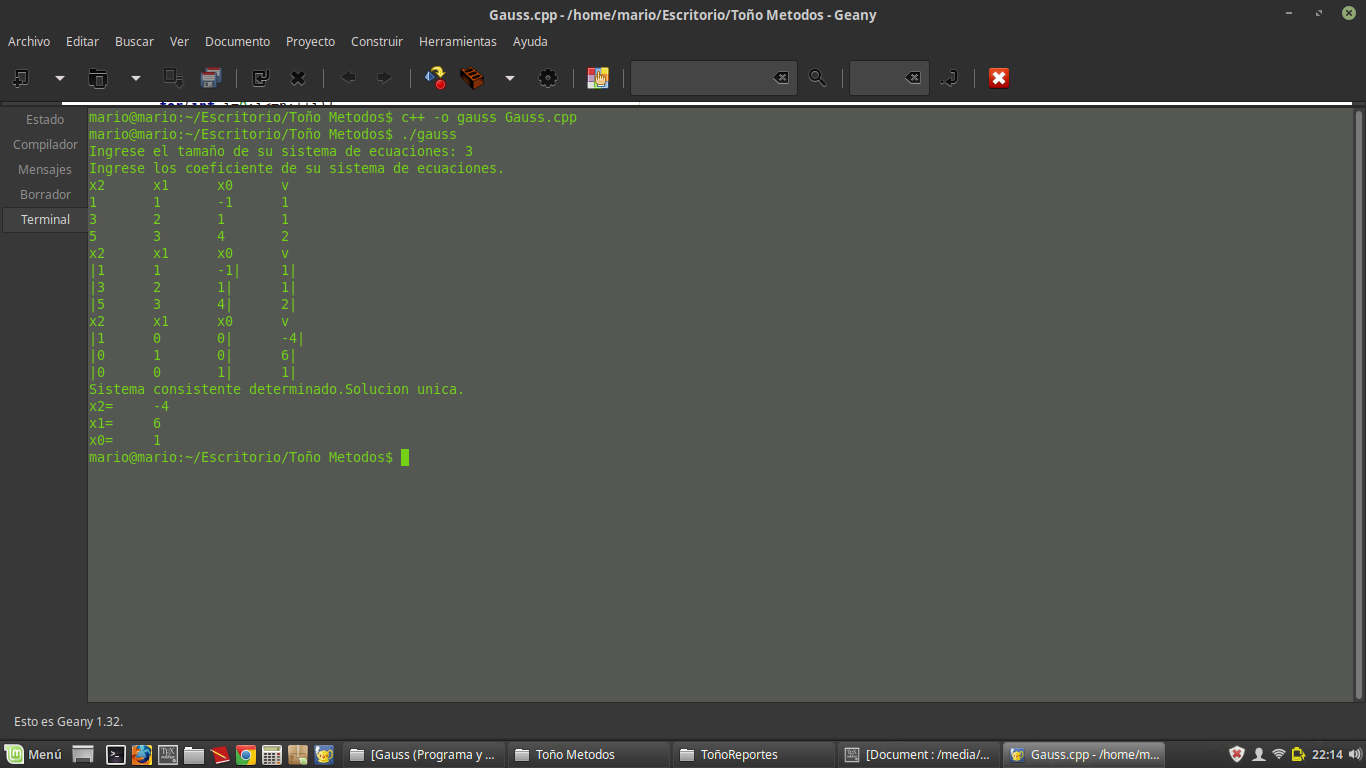
\includegraphics[scale=.125]{Gauss.png}
\caption{Implementacion del metodo de Gauss-Yordan en un programa}
\end{figure}

\section{Ventajas y Desventajas}
\label{sec:Ven}
\textbf{Ventajas}
\\
1.Arroja resultados mas precisos.
\\
2. Las operaciones son mas sencillas que en otros metodos.
\\
3. Otorgan mas datos para poder
\\
\\
\textbf{Desventajas}
\\
1. Es bastante laborioso y es sencillo de equivocarse.
\\
2. Cuando se manejan numeros flotantes, es complicado, su procedimiento.
\\
3. Para la programacion, es complicado programarlo debido a los distinpos tipos de programacion a los cuales se deberian de aplicar al metodo en si.
 
\end{multicols}

\end{document}